\documentclass{article} 
\usepackage{tikz}
\usetikzlibrary{trees}

\begin{document}
\scalebox{1.5}{
    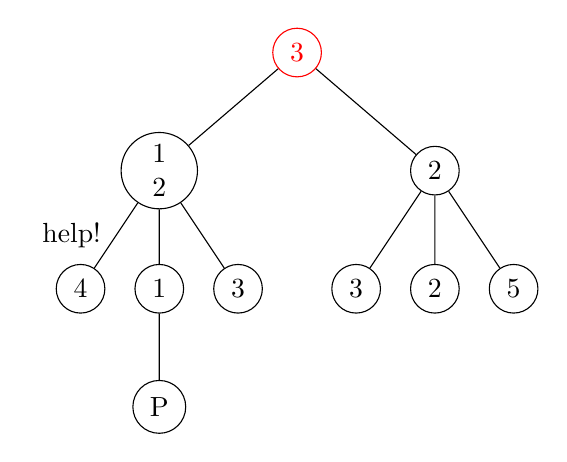
\begin{tikzpicture}[
        level distance=1.5cm,
        level 1/.style={sibling distance=3.5cm},
        level 2/.style={sibling distance=1cm}
    ]

    \tikzstyle{every node}=[circle,draw, align=center]


    \node (root) [red] {3}
        child {
            node {1\\2} 
            child {
                node {4} 
                edge from parent node[left,draw=none] {help!} 
            }
            child { 
                node {1} 
                child { 
                    node {P} 
                }
            }
            child {
                node {3}
            }
        }
        child {
            node {2}
            child {
                node {3}
            }
            child {
                node {2}
            }
            child {
                node {5}
            }
        };

    \end{tikzpicture}
}

\end{document}